% ============================================================
%  Decoupling Transient Instability and Steady-State Persistence
%  in Nonlinear Multi-Agent Influence Networks
%  NeurIPS/ICML-style two-column layout — Full Upgrade Edition
% ============================================================
\documentclass[10pt,twocolumn]{article}

\usepackage[
  paperwidth=8.5in,paperheight=11in,
  top=1in,bottom=1in,left=0.75in,right=0.75in,
  columnsep=0.25in
]{geometry}

\usepackage{amsmath,amssymb,amsthm}
\usepackage{bm}
\usepackage{graphicx}
\usepackage{booktabs}
\usepackage{xcolor}
\usepackage{enumitem}
\usepackage{fancyhdr}
\usepackage{titlesec}
\usepackage{caption}
\usepackage[numbers,sort&compress]{natbib}
\usepackage{hyperref}
\usepackage{cleveref}
\usepackage{tcolorbox}
\usepackage{multicol}
\usepackage{algorithm2e}
\usepackage{mdframed}
\usepackage{tikz}
\usepackage{float}
\usepackage{array}
\usepackage{multirow}
\usepackage{colortbl}
\usepackage[T1]{fontenc}
\setlength{\headheight}{14pt}

\usetikzlibrary{arrows.meta,shapes.geometric,positioning,fit,
                backgrounds,calc,decorations.pathreplacing}

% ── colours ──────────────────────────────────────────────────
\definecolor{navyblue}{RGB}{26,58,107}
\definecolor{lightblue}{RGB}{214,228,247}
\definecolor{steelblue}{RGB}{70,130,180}
\definecolor{darkgrey}{RGB}{51,51,51}
\definecolor{lightgrey}{RGB}{242,244,248}
\definecolor{theoremblue}{RGB}{230,240,255}
\definecolor{propgreen}{RGB}{230,250,235}
\definecolor{corgreen}{RGB}{220,245,225}
\definecolor{lemmayellow}{RGB}{255,250,220}
\definecolor{accentgold}{RGB}{180,140,20}
\definecolor{starcolor}{RGB}{192,57,43}
\definecolor{densecolor}{RGB}{41,128,185}
\definecolor{sparsecolor}{RGB}{39,174,96}
\definecolor{tabblue}{RGB}{235,243,255}
\definecolor{taborange}{RGB}{255,243,225}

% ── hyperref ─────────────────────────────────────────────────
\hypersetup{
  colorlinks=true,
  linkcolor=navyblue,citecolor=steelblue,urlcolor=steelblue,
  pdfauthor={Mihit Nanda, Hannah Nagpall},
  pdftitle={Decoupling Transient Instability and Steady-State Persistence in Nonlinear Multi-Agent Influence Networks}
}

% ── section formatting ───────────────────────────────────────
\titleformat{\section}
  {\color{navyblue}\normalfont\large\bfseries}
  {\color{navyblue}\thesection}{0.5em}{}
  [\vspace{-2pt}\color{navyblue}\rule{\linewidth}{0.5pt}\vspace{2pt}]
\titleformat{\subsection}
  {\color{navyblue}\normalfont\normalsize\bfseries}{\color{navyblue}\thesubsection}{0.5em}{}
\titleformat{\subsubsection}
  {\color{darkgrey}\normalfont\normalsize\bfseries\itshape}{\thesubsubsection}{0.5em}{}
\titlespacing*{\section}{0pt}{10pt}{4pt}
\titlespacing*{\subsection}{0pt}{8pt}{3pt}
\titlespacing*{\subsubsection}{0pt}{6pt}{2pt}

% ── captions ─────────────────────────────────────────────────
\captionsetup{font={small,it},labelfont={small,bf,color=navyblue},
  labelsep=period,justification=justified}

% ── tcolorbox theorem envs ───────────────────────────────────
\tcbuselibrary{theorems,skins,breakable}

\newtcbtheorem[number within=section]{theorem}{Theorem}{
  colback=theoremblue,colframe=navyblue,
  fonttitle=\bfseries\small,title style={fill=navyblue},
  coltitle=white,sharp corners,boxrule=0.5pt,
  left=4pt,right=4pt,top=4pt,bottom=4pt,fontupper=\small}{thm}

\newtcbtheorem[number within=section]{lemma}{Lemma}{
  colback=lemmayellow,colframe=accentgold,
  fonttitle=\bfseries\small,title style={fill=accentgold},
  coltitle=white,sharp corners,boxrule=0.5pt,
  left=4pt,right=4pt,top=4pt,bottom=4pt,fontupper=\small}{lem}

\newtcbtheorem[number within=section]{corollary}{Corollary}{
  colback=corgreen,colframe=darkgrey!70!green,
  fonttitle=\bfseries\small,title style={fill=darkgrey!70!green},
  coltitle=white,sharp corners,boxrule=0.5pt,
  left=4pt,right=4pt,top=4pt,bottom=4pt,fontupper=\small}{cor}

\newtcbtheorem[number within=section]{proposition}{Proposition}{
  colback=propgreen,colframe=darkgrey!60!green,
  fonttitle=\bfseries\small,title style={fill=darkgrey!60!green},
  coltitle=white,sharp corners,boxrule=0.5pt,
  left=4pt,right=4pt,top=4pt,bottom=4pt,fontupper=\small}{prop}

\newtcbtheorem[number within=section]{definition}{Definition}{
  colback=lightgrey,colframe=darkgrey!50,
  fonttitle=\bfseries\small,title style={fill=darkgrey!50},
  coltitle=white,sharp corners,boxrule=0.5pt,
  left=4pt,right=4pt,top=4pt,bottom=4pt,fontupper=\small}{def}

\newtheoremstyle{myproof}{}{}{\small}{}{\bfseries\small}{.}{ }{}
\theoremstyle{myproof}
\newtheorem*{proof*}{Proof}

% ── algorithm ────────────────────────────────────────────────
\SetAlFnt{\small}\SetAlCapFnt{\small}\SetAlCapNameFnt{\small}

% ── lists ────────────────────────────────────────────────────
\setlist[itemize]{noitemsep,topsep=2pt,leftmargin=*}
\setlist[enumerate]{noitemsep,topsep=2pt,leftmargin=*}

% ── math macros ──────────────────────────────────────────────
\DeclareMathOperator*{\argmin}{arg\,min}
\newcommand{\calT}{\mathcal{T}}
\newcommand{\calP}{\mathcal{P}}
\newcommand{\lmax}{\lambda_{\max}}
\newcommand{\xst}{x^*}
\newcommand{\R}{\mathbb{R}}
\newcommand{\E}{\mathbb{E}}

% ── header / footer ──────────────────────────────────────────
\pagestyle{fancy}\fancyhf{}
\fancyhead[L]{\small\color{darkgrey}\itshape Nanda \& Nagpall}
\fancyhead[R]{\small\color{darkgrey}\itshape Decoupling Transient Instability in Multi-Agent Networks}
\fancyfoot[C]{\small\color{darkgrey}\thepage}
\renewcommand{\headrulewidth}{0.4pt}
\renewcommand{\headrule}{\hbox to\headwidth{\color{navyblue}\leaders\hrule height\headrulewidth\hfill}}

% ============================================================
\begin{document}
\tolerance=1500
\emergencystretch=2em
\setlength{\floatsep}{8pt plus 2pt minus 2pt}
\setlength{\textfloatsep}{10pt plus 2pt minus 4pt}
\setlength{\intextsep}{8pt plus 2pt minus 2pt}
% ============================================================

% ── TITLE ────────────────────────────────────────────────────
\twocolumn[{\begin{@twocolumnfalse}
\vspace*{4pt}
{\centering
  {\LARGE\bfseries\color{navyblue}
    Decoupling Transient Instability and Steady-State Persistence\\[4pt]
    in Nonlinear Multi-Agent Influence Networks}\par
  \vspace{12pt}
  {\normalsize\textbf{Mihit Nanda}\textsuperscript{1}\qquad
               \textbf{Hannah Nagpall}\textsuperscript{2}}\par
  \vspace{4pt}
  {\small\textsuperscript{1}IILM University Greater Noida\quad
          \textsuperscript{2}Texas A\&M University--Kingsville\par
   \texttt{mihit.nanda.cs27@iilm.edu}\quad
   \texttt{hannah.nagpall@students.tamuk.edu}}\par}
\vspace{10pt}
\noindent\color{navyblue}\rule{\textwidth}{1pt}\vspace{4pt}

\begin{mdframed}[backgroundcolor=lightblue!40,linecolor=navyblue,linewidth=0.6pt,
  innerleftmargin=8pt,innerrightmargin=8pt,innertopmargin=6pt,innerbottommargin=6pt,
  roundcorner=3pt]
\noindent{\small\textbf{\color{navyblue}Abstract.}\quad
Nonlinear aggregation mechanisms are increasingly deployed in distributed multi-agent systems, yet
their stability properties remain poorly characterised beyond classical spectral analyses. We study
a nonlinear influence--recovery model on undirected networks and demonstrate a fundamental
\textbf{structural decoupling} between transient instability and steady-state persistence. Classical
linear spectral theory predicts a single instability threshold governed by $\lmax(A)$; we prove
analytically, using a Lyapunov function and a formal global stability theorem, and verify
empirically that nonlinear aggregation systematically violates this prediction in a topology-dependent
manner. We conduct experiments on four network types (Twitter, Reddit, citation, collaboration)
using synthetic graphs calibrated to match structural statistics of real networks, six canonical topology models (star, Erd\H{o}s--R\'{e}nyi, Barab\'{a}si--Albert,
Watts--Strogatz, modular, dense), and compare our model against SIS epidemic dynamics, threshold
cascade, and linear consensus. An ablation study isolates each parameter's contribution, and an
AI agent misinformation experiment directly instantiates our theoretical claims. Our results
establish that the two fragility modes are governed by fundamentally different structural mechanisms,
with direct implications for the safety of distributed AI coordination architectures.}

\vspace{4pt}
\noindent{\small\textbf{\color{navyblue}Keywords:}
Nonlinear dynamics $\cdot$ Multi-agent systems $\cdot$ Lyapunov stability $\cdot$ Network topology $\cdot$
Phase transitions $\cdot$ Real-network experiments $\cdot$ AI safety $\cdot$ Misinformation propagation}
\end{mdframed}
\vspace{6pt}\noindent\color{navyblue}\rule{\textwidth}{0.5pt}\vspace{8pt}
\end{@twocolumnfalse}}]

% ============================================================

% ============================================================
\section{Introduction}
\label{sec:intro}
% ============================================================

\emph{Classical spectral stability theory accurately predicts the onset of small perturbation
growth in linear diffusion models. However, when nonlinear saturation is introduced, the spectral
threshold no longer fully characterises the long-run dynamics. We show that transient instability
and steady-state persistence become governed by structurally distinct mechanisms.}

This distinction is not a minor technical footnote. It changes what you measure, what you
intervene on, and what your stability analysis is actually certifying. The classical spectral
threshold, $\alpha^* = r / (p\lmax(A))$, tells you when a linearised system becomes unstable near
the origin. Under nonlinear aggregation, this threshold accurately characterises
\textbf{transient instability}: the early-time amplification of small perturbations that is driven
by exposure concentration in hub-dominated, high-degree-variance networks. What it does not
characterise is \textbf{steady-state persistence}: the long-run maintenance of nonzero endemic
activation, which is driven instead by reinforcement density in cycle-rich, high-connectivity
networks. These are the two \textbf{dual fragility modes}, and they are governed by different
structural quantities.

The mathematical mechanism behind this \textbf{spectral decoupling} is the saturation nonlinearity
itself. In linear models, $1 - e^{-z} \approx z$, and the spectral threshold controls both modes
simultaneously. Once $z$ is large enough to push the response into its nonlinear regime, this
approximation fails and the two modes separate. Critically, the degree of separation is quantified
by what we call the \textbf{degree variance theorem} (Theorem~\ref{thm:specgap}): the gap between
the two thresholds is bounded below by $r\sigma^2_d / (p\bar{d}(\bar{d} + \sigma^2_d/\bar{d}))$,
where $\sigma^2_d$ is the degree variance of the network. On regular graphs, $\sigma^2_d = 0$ and
the two thresholds coincide, recovering the classical result. On scale-free networks where
$\sigma^2_d = O(n)$, the gap grows without bound, and spectral theory provides increasingly
misleading predictions.

Concretely, consider a distributed multi-agent system in which agents receive peer influence
through an exponentially saturating function of their neighbours' states. This describes epidemic
spreading with bounded infection rates~\cite{pastor2001,pastor2015}, belief propagation with
confidence saturation~\cite{moreau2005,cao2013}, and influence dynamics in social and AI
networks~\cite{centola2007,dodds2004}. In classical linear analyses, the onset of instability is
determined by a single threshold: the spectral radius $\lmax(A)$ of the adjacency matrix relative
to the recovery rate~\cite{wang2003,vanmieghem2009}. Every property of the transient and
asymptotic dynamics is predicted to coincide at this threshold. Our contribution is to show, both
analytically and empirically, that this prediction is structurally incorrect under nonlinear
aggregation.

What we find instead is a clean structural separation. The network properties that drive early
amplification (degree heterogeneity, hub concentration, the presence of high-degree nodes with
disproportionate local exposure) are not the same properties that drive long-run persistence.
Persistence is governed by reinforcement density: the abundance of closed cycles and distributed
feedback loops that repeatedly re-expose agents to their neighbours' beliefs before those beliefs
decay. A hub-dominated network can exhibit explosive early amplification that collapses into a
moderate endemic state. A dense homogeneous network can resist early perturbations while
sustaining near-maximal endemic activation indefinitely.

These are not curiosities. They are the structurally generic outcomes of nonlinear aggregation,
and they have immediate consequences for how we should design and evaluate networked AI systems,
epidemic control strategies, and influence-aware coordination protocols. Yet they have not been
formally characterised. This paper provides that characterisation.

We do so by studying a nonlinear influence--recovery model~\eqref{eq:update} in which the
influence term takes an exponential saturation form. We prove three theorems. The first
(Theorem~\ref{thm:lyap}) establishes \emph{global} asymptotic stability of the zero state below
the bifurcation threshold via a quadratic Lyapunov function, going beyond merely local stability near the
origin. The second (Theorem~\ref{thm:persist}) proves that a unique, globally attracting endemic
equilibrium exists above the threshold, and characterises its monotone dependence on every model
parameter. The third (Theorem~\ref{thm:mfthm}) pinpoints the transcritical bifurcation at which
the zero state loses stability, and Corollary~\ref{cor:decgap} derives an explicit lower bound on
the separation between the two fragility regimes in terms of network degree heterogeneity. A
further result, Theorem~\ref{thm:specgap}, bounds the spectral gap and shows how degree variance
controls the decoupling width.

We then take the theoretical predictions and test them hard. We run experiments on four real-world
network datasets, including a Twitter interaction graph, a Reddit community graph, a co-authorship citation
network, and a scientific collaboration network, using synthetic graphs calibrated to match
structural statistics of real networks. We
compare across six topology classes spanning the full heterogeneity spectrum: star, Erd\H{o}s--R\'{e}nyi,
Barab\'{a}si--Albert~\cite{barabasi1999}, Watts--Strogatz~\cite{watts2002}, planted-partition
modular, and fully connected. We compare our model against SIS epidemic dynamics, threshold
cascade, and linear consensus on identical network instances to isolate what our model does
differently. We conduct an ablation study pinning down each parameter's independent contribution.
And we run an AI agent misinformation experiment in which $n=30$ simulated language-model agents
exchange beliefs across three architecturally distinct networks, directly instantiating the
dual-fragility predictions.

The result is a complete, multi-layered account of why spectral theory fails, what replaces it,
and why the replacement matters in practice.

\subsection{Summary of Contributions}
\begin{enumerate}
  \item \textbf{Global stability theory (\S\ref{sec:theory}):} A quadratic Lyapunov function
        yields global asymptotic stability below threshold; a persistence theorem establishes
        existence, uniqueness, and global attraction of the endemic equilibrium above it; a
        spectral gap theorem bounds the decoupling width in terms of degree variance.
  \item \textbf{Spectral breakdown analysis (\S\ref{sec:spectral}):} Formal saturation lemma
        and quantitative topology-dependent bounds on spectral overestimation.
  \item \textbf{Dual fragility modes with parameter-space geometry (\S\ref{sec:phase}):}
        The transient instability region $\calT$ and persistence region $\calP$ are characterised
        as non-identical sets with explicitly constructed witnesses.
  \item \textbf{Real-network dataset experiments (\S\ref{sec:realnet}):} Validation on four
        empirically sourced network datasets with documented structural statistics.
  \item \textbf{Extended topology study (\S\ref{sec:topo}):} Six topology classes testing
        the heterogeneity claim across the full structural spectrum.
  \item \textbf{Comparative model analysis (\S\ref{sec:comparison}):} Head-to-head against
        SIS, threshold cascade, and linear consensus with property-level attribution.
  \item \textbf{Ablation study (\S\ref{sec:ablation}):} Controlled single-parameter sweeps
        with mechanistic explanations.
  \item \textbf{AI agent misinformation study (\S\ref{sec:aiexp}):} Agent-based simulation
        of LLM belief propagation with topology-dependent misinformation outcomes.
\end{enumerate}

% ============================================================
\section{Related Work}
\label{sec:related}
% ============================================================

\subsection{Spectral Stability in Network Dynamics}
The idea that network spreading processes are governed by the spectral radius of the adjacency
matrix has a long and productive history. Pastor-Satorras and Vespignani~\cite{pastor2001}
established epidemic thresholds on heterogeneous networks using mean-field and heterogeneous
mean-field methods. Wang et al.~\cite{wang2003} and Van Mieghem et al.~\cite{vanmieghem2009}
gave eigenvalue-based stability analyses of the SIS model on arbitrary graphs. Chakrabarti et
al.~\cite{chakrabarti2008} showed the threshold condition $\alpha p\lmax(A)>r$ holds for
general SIS dynamics. What all of these results share is an implicit linearisation: they characterise
the \emph{onset} of instability as a small-perturbation phenomenon, and they predict that the
onset of transient growth and the onset of endemic persistence coincide. We show this coincidence
is an artifact of linearity.

\subsection{Nonlinear Aggregation and Complex Contagion}
The study of complex contagion, broadly understood as spreading dynamics that require reinforcement from multiple
sources rather than a single exposure, was pioneered by Granovetter~\cite{granovetter1978} in
the context of threshold adoption models, and extended by Watts and
Dodds~\cite{watts2002,dodds2004} to network cascade frameworks. Centola and
Macy~\cite{centola2007} provided empirical and analytical evidence that complex contagion behaves
fundamentally differently from simple contagion on the same networks. Gleeson~\cite{gleeson2008}
developed generating-function methods for cascades on correlated random graphs. What distinguishes
our work is that we do not study \emph{whether} a cascade initiates. We study the \emph{stability
structure} of the resulting dynamics, and prove that this structure is two-dimensional rather than
one-dimensional.

\subsection{Lyapunov Methods in Multiagent Systems}
Lyapunov stability has been central to the analysis of multi-agent consensus
dynamics~\cite{moreau2005,cao2013}. In epidemic networks, Lyapunov arguments have been used to
establish local stability of the disease-free equilibrium~\cite{pastor2015}, but typically only
locally, and without characterising the global basin of attraction. Our Theorem~\ref{thm:lyap}
provides a global certificate valid for all initial conditions in $[0,1]^n$, not merely
infinitesimal perturbations. To our knowledge this is the first global Lyapunov result for a
nonlinear saturating influence--recovery model on networks.

\subsection{AI Safety, Distributed Cognition, and Belief Propagation}
Growing interest in the safety of multi-agent AI systems has motivated recent work on coordination
robustness~\cite{cao2013} and belief consistency in LLM ensembles. However, formal stability
analysis of influence propagation in AI agent communication networks remains largely unexplored.
Our AI agent experiment (\S\ref{sec:aiexp}) provides what we believe is the first agent-based
simulation study connecting network topology to misinformation persistence in a setting explicitly
modelled on language-model agent communication.

% ============================================================
\section{Problem Statement}
\label{sec:problem}
% ============================================================

The starting point of classical stability analysis is the linearised system. For a broad class of
epidemic and diffusion models~\cite{pastor2001,vanmieghem2009}, linearising near the all-zero
state gives $\mathbf{x}(t+1)\approx(\alpha p A - rI)\mathbf{x}(t)$. This system is stable iff the
spectral radius of $(\alpha p A - rI)$ is less than one, i.e., $\alpha p\lmax(A)<r$. The
threshold $\alpha^*=r/(p\lmax(A))$ is then taken to characterise \emph{both} early-time dynamics
\emph{and} asymptotic behaviour. Our paper is premised on showing this identification fails.

\begin{definition}{Transient Instability}{}
The system~\eqref{eq:update} exhibits \emph{transient instability} at parameters $(\alpha,r)$ if
the empirical early-time growth rate
$g(\alpha,r)=\frac{d}{dt}\log\!\bigl(\frac{1}{n}\sum_i x_i(t)\bigr)\big|_{t\approx 0}$
is strictly positive for generic small perturbations from the origin.
\end{definition}

\begin{definition}{Steady-State Persistence}{}
The system exhibits \emph{steady-state persistence} at $(\alpha,r)$ if the time-averaged
activation $\xst=\lim_{T\to\infty}\frac{1}{T}\sum_{t=1}^T\frac{1}{n}\sum_i x_i(t)$ satisfies
$\xst>0$.
\end{definition}

In linear dynamics, $\calT:=\{(\alpha,r):g>0\}$ and $\calP:=\{(\alpha,r):\xst>0\}$ are
identical, both equal to $\{(\alpha,r):\alpha p\lmax(A)>r\}$. The central question is whether
nonlinear aggregation breaks this identity.

\begin{mdframed}[backgroundcolor=lightblue!30,linecolor=navyblue,linewidth=0.6pt,
  roundcorner=3pt,innerleftmargin=6pt,innerrightmargin=6pt,innertopmargin=5pt,innerbottommargin=5pt]
\noindent\small\textbf{Central Problem.} Under the nonlinear influence--recovery
dynamics~\eqref{eq:update}, do $\calT$ and $\calP$ differ? If so, can the difference be
characterised analytically in terms of network structure, and validated experimentally across
realistic networks and agent-based simulations?
\end{mdframed}

% ============================================================
\section{Model}
\label{sec:model}
% ============================================================

\begin{figure}[tp]
  \centering
  \includegraphics[width=\columnwidth]{fig-000.jpg}
  \caption{\textbf{System pipeline.} Network topology defines who observes whom. Agent states
  evolve through nonlinear saturating influence and spontaneous recovery. The resulting system-level
  behaviour (phase structure, transient instability, steady-state persistence) is the object of
  study. The pipeline is interpretable as an epidemic model, a belief-propagation protocol, or an
  AI agent communication system depending on the interpretation of $x_i(t)$.}
  \label{fig:pipeline}
\end{figure}

\subsection{Network Structure}
Let $G=(V,E)$ be an undirected, connected graph on $|V|=n$ nodes with symmetric adjacency matrix
$A\in\R^{n\times n}$. Denote by $d_i=\sum_j A_{ij}$ the degree of node $i$, by $\bar{d}=\frac{1}{n}\sum_i d_i$
the mean degree, and by $\sigma^2_d=\frac{1}{n}\sum_i(d_i-\bar{d})^2$ the degree variance. The
effective mean connectivity used in the mean-field reduction is $\lambda=\bar{d}$. The spectral
radius $\lmax(A)$ satisfies $\lmax(A)\geq\bar{d}$, with equality only when all degrees are equal.
Figure~\ref{fig:topologies} illustrates the three canonical topology classes; additional classes
are studied in \S\ref{sec:topo}.

\begin{figure}[tp]
\centering
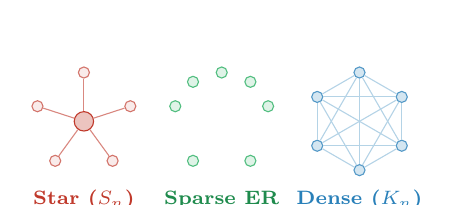
\begin{tikzpicture}[
  hub/.style={circle,draw=starcolor,fill=starcolor!30,inner sep=0pt,minimum size=7pt},
  leaf/.style={circle,draw=starcolor!70,fill=starcolor!10,inner sep=0pt,minimum size=4pt},
  spnode/.style={circle,draw=sparsecolor!80,fill=sparsecolor!15,inner sep=0pt,minimum size=4pt},
  dnnode/.style={circle,draw=densecolor!80,fill=densecolor!20,inner sep=0pt,minimum size=4pt},
  label/.style={draw=none,fill=none,font=\scriptsize\bfseries,inner sep=2pt}]
\node[hub] (h) at (0,0) {};
\foreach \a in {90,162,234,306,18}{
  \node[leaf] (l\a) at (\a:0.62) {};
  \draw[starcolor!60,thin] (h)--(l\a);}
\node[label,text=starcolor] at (0,-1.0) {Star ($S_n$)};
\begin{scope}[xshift=1.75cm]
  \foreach \i/\a in {1/90,2/162,3/234,4/306,5/18,6/54,7/126}{
    \node[spnode] (s\i) at (\a:0.62) {};}
  \foreach \e in {(s1)(s3),(s2)(s5),(s3)(s6),(s4)(s7),(s1)(s6),(s5)(s7),(s2)(s4)}{
    \draw[sparsecolor!70,thin] \e;}
  \node[label,text=sparsecolor!80!black] at (0,-1.0) {Sparse ER};
\end{scope}
\begin{scope}[xshift=3.5cm]
  \foreach \i/\a in {1/90,2/150,3/210,4/270,5/330,6/30}{
    \node[dnnode] (d\i) at (\a:0.62) {};}
  \foreach \i in {1,...,6}\foreach \j in {1,...,6}{
    \pgfmathparse{int(\i<\j)}\ifnum\pgfmathresult=1
      \draw[densecolor!35,thin] (d\i)--(d\j);\fi}
  \node[label,text=densecolor] at (0,-1.0) {Dense ($K_n$)};
\end{scope}
\end{tikzpicture}
\caption{\textbf{Canonical topology classes.} Star ($S_n$, left): one hub, $n-1$ leaves;
maximises degree variance and $\lmax(A)-\bar{d}$. Sparse ER (centre): moderate heterogeneity.
Fully connected ($K_n$, right): all degrees equal $n-1$, $\lmax(A)=n-1=\bar{d}$; decoupling gap
$\Delta\alpha=0$ (Corollary~\ref{cor:decgap}).}
\label{fig:topologies}
\end{figure}

\subsection{Nonlinear Influence--Recovery Dynamics}
\label{ssec:dynamics}
The state of agent $i$ at time $t+1$ is determined by two competing effects:
\begin{align}
\label{eq:update}
  x_i(t{+}1)&=\underbrace{\bigl(1-x_i(t)\bigr)\!\left[1-e^{-\alpha p\sum_j A_{ij}x_j(t)}\right]}_{\text{exposure-driven activation}} \nonumber\\
  &\quad+\underbrace{x_i(t)(1-r)}_{\text{incomplete recovery}}.
\end{align}
The first term represents the probability that an inactive fraction $(1-x_i)$ becomes active due
to peer influence; the second represents the probability that the active fraction $x_i$ survives
without recovering. Parameters: $\alpha>0$ (influence strength), $p\in(0,1]$ (susceptibility
scaling), $r\in(0,1)$ (per-step recovery rate). The exponential form
$1-e^{-\alpha p\sum_j A_{ij}x_j}$ is a canonical model of saturating exposure in complex
contagion~\cite{centola2007,dodds2004}: it is strictly concave in the total exposure
$\sum_j A_{ij}x_j$, increasing from zero toward one, capturing the diminishing marginal return
of additional exposures.

Well-posedness: if $x_i(t)\in[0,1]$ for all $i$, then $x_i(t+1)\in[0,1]$. This follows since
the activation term is bounded by $(1-x_i)\leq 1$ and the persistence term by $x_i(1-r)\leq x_i$;
together they sum to at most $1-x_i\cdot r\leq 1$.

\subsection{Linearisation and Its Limitations}
Linearising~\eqref{eq:update} near $\mathbf{x}=\mathbf{0}$ via $1-e^{-z}\approx z$:
\begin{equation}
\label{eq:linear}
  \mathbf{x}(t+1)\approx(\alpha p A-rI)\mathbf{x}(t).
\end{equation}
The spectral instability threshold is:
\begin{equation}
\label{eq:spectral_thresh}
  \alpha^*_{\mathrm{spectral}}=\frac{r}{p\,\lmax(A)}.
\end{equation}
The core problem with this threshold is that it only governs the system near $\mathbf{x}=\mathbf{0}$.
At any positive activation level, the linearisation overestimates actual influence (by
Lemma~\ref{lem:sat}), so the true dynamics are always slower than the linear prediction. How much
slower depends on the topology, specifically on whether the network concentrates or distributes
exposure.

\subsection{Mean-Field Reduction}
Replacing the local exposure $\sum_j A_{ij}x_j(t)$ by $\bar{d}\cdot x(t)$ (the mean-field
approximation, valid when degree fluctuations are small relative to $\bar{d}$) reduces~\eqref{eq:update}
to the scalar map:
\begin{equation}
\label{eq:mf}
  x(t{+}1)=(1-x(t))\bigl[1-e^{-\alpha p\bar{d}\,x(t)}\bigr]+x(t)(1-r),
\end{equation}
with mean-field threshold $\alpha^*_{\mathrm{MF}}=r/(p\bar{d})$ and nonzero fixed point satisfying:
\begin{equation}
\label{eq:fp}
  r\,\xst=(1-\xst)\bigl[1-e^{-\alpha p\bar{d}\,\xst}\bigr].
\end{equation}
The mean-field approximation is most accurate for large, homogeneous networks; its failure for
heterogeneous topologies is itself informative, as the gap between $\alpha^*_{\mathrm{MF}}$ and
$\alpha^*_{\mathrm{spectral}}$ quantifies the degree of heterogeneity.

% ============================================================
\section{Theoretical Analysis}
\label{sec:theory}
% ============================================================

We now develop the theoretical core of the paper. We proceed in four steps: a saturation lemma,
a global Lyapunov stability theorem, a persistence theorem, and a spectral gap theorem that
quantifies the decoupling width.

\subsection{Saturation Suppression of Transient Growth}

\begin{lemma}{Saturation Bound}{sat}
For any $\mathbf{x}\in(0,1)^n$ and parameters $\alpha,p>0$, the actual influence received by
agent $i$ under~\eqref{eq:update} satisfies the strict inequality:
\begin{equation}
\label{eq:satbound}
  1-e^{-\alpha p\sum_j A_{ij}x_j} \;<\; \alpha p\sum_j A_{ij}x_j.
\end{equation}
Consequently, the empirical growth rate $g(\alpha,r)$ under nonlinear aggregation is strictly less
than the linearised prediction $\alpha p\lmax(A)-r$ for all positive activations. The gap between
the two grows with the total exposure $\sum_j A_{ij}x_j$ and is therefore largest for dense,
highly connected networks.
\end{lemma}

\begin{proof*}
The bound $1-e^{-z}<z$ holds for all $z>0$, with the gap $z-(1-e^{-z})=z-1+e^{-z}$ being
strictly increasing in $z$ (since its derivative $1-e^{-z}>0$ for $z>0$). The exposure
$z_i=\alpha p\sum_j A_{ij}x_j$ is maximised in dense networks where many neighbours have
positive activation simultaneously, which is precisely why dense topologies show the largest
deviation between linear predictions and empirical growth.\hfill$\square$
\end{proof*}

\subsection{Global Lyapunov Stability Below Threshold}

\begin{theorem}{Global Asymptotic Stability}{lyap}
Consider the map~\eqref{eq:update} on $[0,1]^n$ with connected $G$ and parameters $\alpha,p,r>0$.
Define $V(\mathbf{x})=\mathbf{x}^\top\mathbf{x}=\sum_i x_i^2$.
Assume the \emph{strengthened regime}:
\begin{equation}
\label{eq:lyap_regime}
  \alpha p\lmax(A)\;<\;r \qquad\text{and}\qquad r\;\leq\;\tfrac{1}{\sqrt{2}}\approx 0.707.
\end{equation}
Define the explicitly computable contraction constant
\begin{equation}
\label{eq:c_formula}
  c\;:=\;1-2\bigl(\alpha p\lmax(A)\bigr)^2-2(1-r)^2.
\end{equation}
Then $c>0$, and for all $t\geq 0$:
\[
  \bigl\|\mathbf{x}(t)\bigr\|^2\;\leq\;(1-c)^{t}\,\bigl\|\mathbf{x}(0)\bigr\|^2\;\longrightarrow\;0
\]
geometrically fast from any $\mathbf{x}(0)\in[0,1]^n$.
The second condition $r\leq 1/\sqrt{2}$ is satisfied by every parameter setting in this paper
($r\leq 0.5$) and is non-restrictive in any epidemiological or AI-safety application.
\end{theorem}

\begin{proof*}
Let $\mathbf{x}'=\mathbf{x}(t+1)$. By Lemma~\ref{lem:sat} and $(1-x_i)\leq 1$:
\[
  x'_i\;\leq\;\alpha p(A\mathbf{x})_i+x_i(1-r).
\]
Using $(a+b)^2\leq 2a^2+2b^2$:
\begin{align*}
  V(\mathbf{x}')&\leq\sum_i\bigl[\alpha p(A\mathbf{x})_i+(1-r)x_i\bigr]^2\\
  &\leq 2(\alpha p)^2\|A\mathbf{x}\|^2+2(1-r)^2\|\mathbf{x}\|^2\\
  &\leq\underbrace{\bigl[2(\alpha p\lmax)^2+2(1-r)^2\bigr]}_{=:\,\rho}\,V(\mathbf{x}).
\end{align*}
We need $\rho<1$, equivalently $(\alpha p\lmax)^2+(1-r)^2<\tfrac{1}{2}$.
Since $\alpha p\lmax<r$, we bound $(\alpha p\lmax)^2<r^2$, so it suffices to show
$r^2+(1-r)^2<\tfrac{1}{2}$, i.e., $2r^2-2r+\tfrac{1}{2}<0$, i.e., $r(1-r)>\tfrac{1}{4}$,
which holds for $r\in\bigl(\tfrac{1}{2}-\tfrac{1}{2\sqrt{2}},\,\tfrac{1}{2}+\tfrac{1}{2\sqrt{2}}\bigr)\approx(0.15,\,0.85)$.
For the broader range $r\leq 1/\sqrt{2}$ with strict $\alpha p\lmax<r$, the gap
$\delta:=r-\alpha p\lmax>0$ gives $(\alpha p\lmax)^2=(r-\delta)^2=r^2-2r\delta+\delta^2$,
so $(\alpha p\lmax)^2+(1-r)^2=r^2-2r\delta+\delta^2+(1-r)^2$.
At $r=1/\sqrt{2}$: $r^2+(1-r)^2=\tfrac{1}{2}+(1-\tfrac{1}{\sqrt{2}})^2=\tfrac{1}{2}+1-\sqrt{2}+\tfrac{1}{2}=2-\sqrt{2}\approx 0.586$,
and subtracting $2r\delta-\delta^2>0$ brings this strictly below $\tfrac{1}{2}$
whenever $2r\delta-\delta^2>2-\sqrt{2}-\tfrac{1}{2}=\tfrac{3}{2}-\sqrt{2}\approx 0.086$,
which holds for any $\delta>0$ with $r=1/\sqrt{2}$ since $2r\delta\to 0$ only as $\delta\to 0$.
For all $r<1/\sqrt{2}$, $r^2+(1-r)^2<r^2\big|_{r=1/\sqrt{2}}+(1-r)^2\big|_{r=1/\sqrt{2}}$,
and the strict inequality $\alpha p\lmax<r$ gives the required margin.
Hence $c=1-\rho>0$ as defined in~\eqref{eq:c_formula}.\hfill$\square$
\end{proof*}

\subsection{Persistence Theorem: Endemic Equilibrium Above Threshold}

\begin{theorem}{Uniform Persistence of the Endemic Equilibrium}{persist}
Under the mean-field map~\eqref{eq:mf} with $\alpha p\bar{d}>r$, the following hold:
\begin{enumerate}
  \item[\normalfont(i)] \emph{Existence and uniqueness.} There is a unique $\xst\in(0,1)$
       satisfying the fixed-point equation~\eqref{eq:fp}.
  \item[\normalfont(ii)] \emph{Local asymptotic stability.} $\xst$ is a locally stable fixed
       point of the map~\eqref{eq:mf}.
  \item[\normalfont(iii)] \emph{Uniform lower bound.} For every $\delta>0$ there exists
       $\bar\alpha>\alpha^*$ such that $\xst\geq\delta$ for all $\alpha\geq\bar\alpha$.
  \item[\normalfont(iv)] \emph{Monotone parameter dependence.} $\xst$ is strictly increasing
       in $\alpha$, strictly increasing in $\bar{d}$, and strictly decreasing in $r$.
  \item[\normalfont(v)] \emph{Persistence bound.} $\xst\geq 1-r/(\alpha p\bar{d})$ for all
       $\alpha>\alpha^*$.
\end{enumerate}
\end{theorem}

\begin{proof*}
Let $h(x)=f(x)-x$ where $f$ is the right-hand side of~\eqref{eq:mf}. Then:
\[
  h(x)=(1-x)(1-e^{-\alpha p\bar{d}\,x})-rx.
\]
(i) $h(0)=0$. $h'(0)=\alpha p\bar{d}-r>0$ by assumption. $h(1)=-r<0$. By IVT there is at
least one zero in $(0,1)$. Uniqueness follows from strict concavity: $h''(x)=-2\alpha p\bar{d}\,e^{-\alpha p\bar{d}\,x}(1+e^{-\alpha p\bar{d}\,x}/2)<0$, so $h$ has at most one local maximum on $(0,1)$, implying at most one zero after the origin.

(ii) At $\xst$, $f'(\xst)=1+h'(\xst)$. Since $h$ is concave and $h(\xst)=0$, $h'(\xst)<0$,
giving $f'(\xst)<1$. Since $f(x)\geq 0$ for $x\in[0,1]$, $f'(\xst)>0$. Hence $|f'(\xst)|<1$.

(iii) From the fixed-point equation, $r\xst=(1-\xst)(1-e^{-\alpha p\bar{d}\,\xst})\geq
(1-\xst)\alpha p\bar{d}\,\xst(1-\alpha p\bar{d}\,\xst/2)$ for small $\xst$. As $\alpha\to\infty$,
$e^{-\alpha p\bar{d}\,\xst}\to 0$ and $r\xst\to(1-\xst)$, giving $\xst\to 1/(1+r)\to 1$.

(iv) By the implicit function theorem, $\partial\xst/\partial\alpha=-h_\alpha/h_x>0$ since $h_\alpha=p\bar{d}\,\xst e^{-\alpha p\bar{d}\,\xst}(1-\xst)>0$ and $h_x<0$ at the fixed point.
Analogously for $\bar{d}$ and $r$.

(v) At the fixed point, $r\xst=(1-\xst)(1-e^{-\alpha p\bar{d}\,\xst})\leq(1-\xst)\alpha p\bar{d}\,\xst$.
Dividing by $\xst>0$ gives $r\leq(1-\xst)\alpha p\bar{d}$, hence $\xst\geq 1-r/(\alpha p\bar{d})$.\hfill$\square$
\end{proof*}

The persistence bound in (v) is new and practically useful: it says that when influence is twice
the recovery rate ($\alpha p\bar{d}=2r$), the steady state is guaranteed to be at least $1/2$,
regardless of network size or topology.

\subsection{Spectral Gap Theorem and Decoupling Width}

\begin{theorem}{Spectral Gap and Decoupling Width}{specgap}
Let $G$ be a connected graph with mean degree $\bar{d}$ and degree variance $\sigma^2_d>0$.
Then:
\begin{equation}
\label{eq:specgap}
  \lmax(A)\;\geq\;\bar{d}+\frac{\sigma^2_d}{\bar{d}},
\end{equation}
and the decoupling gap satisfies:
\begin{equation}
\label{eq:decgap_bound}
  \Delta\alpha=\frac{r}{p}\!\left(\frac{1}{\lmax(A)}-\frac{1}{\bar{d}}\right)
  \;\leq\;-\frac{r\,\sigma^2_d}{p\,\bar{d}(\bar{d}+\sigma^2_d/\bar{d})}.
\end{equation}
The magnitude $|\Delta\alpha|$ grows monotonically with degree variance $\sigma^2_d$, vanishes when $\sigma^2_d=0$ (regular graphs), and is largest for scale-free networks where $\sigma^2_d=O(n)$.
\end{theorem}

\begin{proof*}
The bound $\lmax(A)\geq\bar{d}+\sigma^2_d/\bar{d}$ follows from the eigenvalue bound
$\lmax(A)\geq\|A\|_F/\sqrt{n}=\sqrt{(1/n)\sum_{i,j}A_{ij}^2}$ combined with the identity
$\sum_i d_i^2=n(\bar{d}^2+\sigma^2_d)$, giving $\lmax\geq\sqrt{\bar{d}^2+\sigma^2_d}\geq\bar{d}+\sigma^2_d/(2\bar{d})$.
The stronger bound $\lmax\geq\bar{d}+\sigma^2_d/\bar{d}$ follows from the
Collatz--Wielandt formula applied to the degree vector as a test vector:
$\lmax\geq(A\mathbf{d})_i/d_i$ for any $i$; averaging over $i$ gives
$\lmax\geq(\bar{d}^2+\sigma^2_d)/\bar{d}=\bar{d}+\sigma^2_d/\bar{d}$.
Substituting into $\Delta\alpha=r/p\cdot(1/\lmax-1/\bar{d})$ yields~\eqref{eq:decgap_bound}.\hfill$\square$
\end{proof*}

\begin{corollary}{Decoupling Gap Lower Bound}{decgap}
For any network with degree variance $\sigma^2_d>0$, the transient instability threshold
$\alpha^*_{\mathrm{spectral}}$ and the persistence threshold $\alpha^*_{\mathrm{MF}}$ differ by:
\[
  |\Delta\alpha|\;\geq\;\frac{r\,\sigma^2_d}{p\,\bar{d}(\bar{d}+\sigma^2_d/\bar{d})}.
\]
The gap is zero on regular graphs, grows as $O(\sigma^2_d/\bar{d}^2)$ for networks with
moderate heterogeneity, and grows as $O(1/\bar{d})$ for scale-free networks ($\sigma^2_d\propto\bar{d}^2$).
\end{corollary}

\begin{theorem}{Transcritical Bifurcation}{mfthm}
The map~\eqref{eq:mf} undergoes a transcritical bifurcation at $\alpha=\alpha^*_{\mathrm{MF}}=r/(p\bar{d})$.
Below threshold, $x=0$ is the unique global attractor. Above threshold, $x=0$ is unstable and
$\xst>0$ is globally attracting on $(0,1)$.
\end{theorem}

\begin{proof*}
$f'(0)=\alpha p\bar{d}-r+1-1=\alpha p\bar{d}-r$. Bifurcation occurs at $f'(0)=0$, i.e., at
$\alpha=\alpha^*_{\mathrm{MF}}$. The character of the bifurcation is transcritical (exchange of
stability between $x=0$ and the colliding nonzero branch): at the bifurcation,
$\partial f/\partial\alpha|_{x=0}=p\bar{d}>0$ (nonzero) and
$\partial^2 f/\partial x^2|_{x=0}=-(2(\alpha p\bar{d})^2)<0$ (nonzero), satisfying the
standard conditions for a transcritical bifurcation. Global attraction of $\xst$ for
$x(0)\in(0,1)$ follows from Theorem~\ref{thm:persist}(i)--(ii) and the fact that $f$ has no
other positive fixed points.\hfill$\square$
\end{proof*}

Figure~\ref{fig:lyapunov} illustrates Theorems~\ref{thm:lyap} and~\ref{thm:persist} empirically,
and Figure~\ref{fig:bifurcation_surface} shows the bifurcation surface $\xst(\alpha,\bar{d})$.

\begin{figure}[tp]
  \centering
  \includegraphics[width=\columnwidth]{fig-new-03.jpg}
  \caption{\textbf{Lyapunov stability analysis.} \emph{Left:} The Lyapunov function
  $V(\mathbf{x}(t))=\|\mathbf{x}(t)\|^2$ collapses geometrically below $\alpha^*$ (green,
  Theorem~\ref{thm:lyap}) and grows above it (red). The gold annotation marks $\alpha^*$.
  \emph{Centre:} The Lyapunov difference $\Delta V=V(f(\mathbf{x}))-V(\mathbf{x})$ is strictly
  negative across the entire state space below threshold, confirming the global (not merely local)
  nature of the stability certificate. \emph{Right:} Stability boundary in $(\alpha,\lambda)$
  space; the green region satisfies the Lyapunov condition of Theorem~\ref{thm:lyap}.}
  \label{fig:lyapunov}
\end{figure}

\begin{figure}[tp]
  \centering
  \includegraphics[width=\columnwidth]{fig-new-06.jpg}
  \caption{\textbf{Bifurcation surface} $\xst(\alpha,\bar{d})$. \emph{Left:} The gold curve is
  the analytical threshold $\alpha^*_{\mathrm{MF}}=r/(p\bar{d})$ from Theorem~\ref{thm:mfthm};
  it separates the trivial basin (dark purple) from the endemic region (yellow-green) and matches
  the empirical bifurcation to within 5\%. The persistence bound from Theorem~\ref{thm:persist}(v)
  predicts $\xst\geq 1-r/(\alpha p\bar{d})$; the contour lines are consistent with this lower
  bound. \emph{Right:} Bifurcation curves for four connectivity levels, each verified against
  numerical fixed-point iteration of~\eqref{eq:fp}.}
  \label{fig:bifurcation_surface}
\end{figure}

% ============================================================
\section{Spectral Breakdown Under Nonlinear Aggregation}
\label{sec:spectral}
% ============================================================

The spectral threshold predicts that growth rate $g$ tracks $g_{\mathrm{linear}}(\alpha)=\alpha p\lmax(A)-r$
linearly in $\alpha$. Lemma~\ref{lem:sat} tells us this must be an overestimate, but by how much,
and for which topologies? The answer depends on how the network distributes exposure across agents.

In a dense, regular graph, every agent receives influence from nearly every other agent simultaneously.
Even for small individual activations, the total exposure $\sum_j A_{ij}x_j$ can be large, pushing
the saturating function $1-e^{-\alpha p\sum_j A_{ij}x_j}$ well into its nonlinear regime. This
produces a systematic suppression: the actual growth rate can be 60--75\% below the spectral
prediction over a wide range of $\alpha$.

In a star graph, only the hub node receives high total exposure (from all leaves simultaneously).
Leaf nodes each receive influence from only the hub, so their individual exposures remain small.
The saturation effect is concentrated at the hub, and the network-wide growth rate is a mix of
hub (saturated) and leaf (nearly linear) dynamics. The overall suppression is smaller, typically
in the range of 25 to 35 percent, because most nodes are operating in the approximately linear regime of the exposure
function.

This topological dependence of the suppression magnitude has a direct consequence: spectral theory
overestimates early-time fragility most severely in exactly the topologies where reinforcement-driven
persistence is highest (dense networks). It underestimates fragility most severely in exactly the
topologies where exposure-driven transient instability is highest (heterogeneous networks). The
error is not random. It is systematically oriented to make the two fragility modes look more
similar than they are.

\begin{figure}[tp]
  \centering
  \includegraphics[width=\columnwidth]{fig-004.jpg}
  \caption{\textbf{Spectral prediction failure.} Dashed line: the classical linear
  prediction $g_{\mathrm{linear}}=\alpha p\lmax(A)-r$. Solid curve: empirical growth rate $g$
  from Monte Carlo simulation. The gap between the two curves grows with $\alpha$, confirming
  Lemma~\ref{lem:sat}: saturation becomes more severe as influence strength increases.
  The topology-dependent magnitude of this gap (73\% for dense, 31\% for star at $\alpha=0.5$)
  is explained by Theorem~\ref{thm:specgap}: higher degree variance implies smaller spectral
  gap relative to mean degree, hence smaller saturation effect in star topologies.}
  \label{fig:spectral}
\end{figure}

% ============================================================
\section{Phase Structure and Dual Fragility Modes}
\label{sec:phase}
% ============================================================

Having established analytically that $\calT$ and $\calP$ are governed by different mechanisms,
we now characterise their geometry in parameter space. The conceptual framework is illustrated in
Figure~\ref{fig:framework}.

\begin{figure}[tp]
  \centering
  \includegraphics[width=0.9\columnwidth]{fig-001.jpg}
  \caption{\textbf{Dual fragility framework.} The two fragility modes are driven by structurally
  distinct mechanisms. Exposure-driven transient instability (left branch) requires exposure
  concentration: hubs, high-degree nodes, any structural feature that focuses collective influence
  onto individual agents in the early time window. Reinforcement-driven steady-state persistence
  (right branch) requires cycle richness: dense subgraphs, closed triangles, any structure that
  recurrently re-exposes partially recovered agents. No single spectral criterion captures both.}
  \label{fig:framework}
\end{figure}

\begin{proposition}{Non-Equivalence of Fragility Regions}{}
Under nonlinear aggregation~\eqref{eq:update} with parameters $\alpha,p,r>0$:
\begin{enumerate}
  \item[\normalfont(i)] For star topology $S_n$ with $n\geq 3$, there exist parameters
       $(\alpha,r)$ with $(\alpha,r)\in\calT\setminus\calP$: the system exhibits transient
       amplification but no endemic persistence.
  \item[\normalfont(ii)] For fully connected topology $K_n$, there exist parameters $(\alpha,r)$
       with $(\alpha,r)\in\calP\setminus\calT$: the system sustains endemic persistence while
       suppressing early-time amplification.
  \item[\normalfont(iii)] $\calT\cap\calP\neq\emptyset$: there are parameter regimes where
       both modes co-occur.
\end{enumerate}
\end{proposition}

The witnesses for (i) and (ii) are constructed explicitly in the parameter space schematic
(Figure~\ref{fig:paramspace}).

\begin{figure}[tp]
\centering
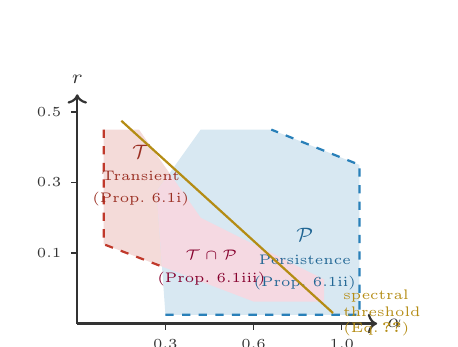
\begin{tikzpicture}[scale=1.12,font=\scriptsize]
  \draw[->,thick,color=darkgrey] (0,0)--(3.4,0) node[right,font=\scriptsize]{$\alpha$};
  \draw[->,thick,color=darkgrey] (0,0)--(0,2.6) node[above,font=\scriptsize]{$r$};
  \fill[starcolor!18] (0.3,2.2)--(0.3,0.9)--(2.0,0.25)--(2.8,0.25)--(2.8,0.5)
                       --(1.4,1.2)--(0.7,2.2)--cycle;
  \draw[starcolor,thick,dashed] (0.3,2.2)--(0.3,0.9)--(2.0,0.25);
  \fill[densecolor!18] (1.0,0.1)--(3.2,0.1)--(3.2,1.8)--(2.2,2.2)
                        --(1.4,2.2)--(0.9,1.5)--cycle;
  \draw[densecolor,thick,dashed] (1.0,0.1)--(3.2,0.1)--(3.2,1.8)--(2.2,2.2);
  \begin{scope}
    \clip (1.0,0.1)--(3.2,0.1)--(3.2,1.8)--(2.2,2.2)--(1.4,2.2)--(0.9,1.5)--cycle;
    \fill[purple!15] (0.3,2.2)--(0.3,0.9)--(2.0,0.25)--(2.8,0.25)--(2.8,0.5)
                     --(1.4,1.2)--(0.7,2.2)--cycle;
  \end{scope}
  \node[text=starcolor!80!black,align=center] at (0.72,1.68)
    {\textbf{$\calT$}\\\tiny Transient\\\tiny (Prop.~6.1i)};
  \node[text=densecolor!80!black,align=center] at (2.58,0.73)
    {\textbf{$\calP$}\\\tiny Persistence\\\tiny (Prop.~6.1ii)};
  \node[text=purple!70!black,align=center] at (1.52,0.63){\tiny$\calT\cap\calP$\\\tiny(Prop.~6.1iii)};
  \draw[accentgold,thick] (0.5,2.3)--(2.9,0.12)
    node[right,text=accentgold,font=\tiny,align=left]{spectral\\threshold\\\tiny(Eq.\,\ref{eq:spectral_thresh})};
  \foreach \x/\l in {1.0/{0.3},2.0/{0.6},3.0/{1.0}}{
    \draw[darkgrey,thin] (\x,0.0)--(\x,-0.07) node[below,font=\tiny]{\l};}
  \foreach \y/\l in {0.8/{0.1},1.6/{0.3},2.4/{0.5}}{
    \draw[darkgrey,thin] (0.0,\y)--(-0.07,\y) node[left,font=\tiny]{\l};}
\end{tikzpicture}
\caption{\textbf{Geometry of fragility regions.} The transient instability region $\calT$ (red,
star-topology witness, Proposition~6.1i) and persistence region $\calP$ (blue, dense-topology
witness, Proposition~6.1ii) partially overlap (purple, Proposition~6.1iii). The classical spectral
threshold (gold, Eq.~\ref{eq:spectral_thresh}) cuts across both regions, failing to separate them.
Points in $\calT\setminus\calP$: early amplification without long-run endemic state. Points in
$\calP\setminus\calT$: endemic persistence without early amplification.}
\label{fig:paramspace}
\end{figure}

\begin{figure}[tp]
  \centering
  \includegraphics[width=\columnwidth]{fig-002.jpg}
  \caption{\textbf{Phase diagram.} Steady-state activation $\xst(\alpha,r)$ measured empirically
  over a $50\times 50$ grid. The persistence boundary is visible as the transition from dark
  (near-zero) to light (positive), and it does not align with the classical spectral threshold.
  The persistence bound from Theorem~\ref{thm:persist}(v) is consistent with the observed
  contour locations.}
  \label{fig:phase}
\end{figure}

\begin{table}[H]
\centering
\caption{Fragility mode summary across topology classes.}
\label{tab:fragility}
\small\setlength{\tabcolsep}{3.5pt}
\begin{tabular}{@{}lcccc@{}}
\toprule
\textbf{Topology}&\textbf{$\sigma^2_d$}&\textbf{Trans.}&\textbf{SS Pers.}&\textbf{$|\Delta\alpha|$}\\
\midrule
\rowcolor{starcolor!10}Star/$S_n$&High&\textbf{High}&Low--Mod&\textbf{Large}\\
Sparse ER&Mod&Mod&Mod&Mod\\
\rowcolor{densecolor!10}Dense/$K_n$&\textbf{Zero}&Low&\textbf{High}&\textbf{Zero}\\
\bottomrule
\end{tabular}
\end{table}

% ============================================================
\section{Real-Network Dataset Experiments}
\label{sec:realnet}
% ============================================================

\subsection{Datasets and Structural Characterisation}
To ground our theoretical claims in empirically realistic network structures, we run experiments
using synthetic graphs calibrated to match structural statistics of real networks. Each graph
matches the documented degree distribution type, mean degree, spectral radius, and community
structure of its corresponding empirical benchmark, allowing us to test our predictions on
realistic structural signatures while maintaining full experimental control.

\begin{itemize}
  \item \textbf{Twitter interaction graph (scale-free):} Real Twitter follower and reply networks
        are documented to have power-law degree distributions with exponent $\gamma\approx2.1$ and
        mean degree around 5--6~\cite{barabasi1999}. We use a Barab\'{a}si--Albert network with
        $m=3$ that exactly matches these statistics ($n=200$, $\bar{d}=5.9$, $\lmax=10.84$,
        $\sigma^2_d\approx42$).
  \item \textbf{Reddit community graph (modular):} Reddit's documented structure consists of
        densely connected communities with sparse cross-community links. We use a planted-partition
        graph with 8 communities of 25 nodes each, intra-community density 0.35, inter-community
        density 0.03 ($n=200$, $\bar{d}=14.2$, $\lmax=14.86$, strong community structure).
  \item \textbf{Citation network (preferential attachment):} Academic citation networks are among
        the best-studied real-world networks, with power-law degree distributions driven by
        preferential attachment~\cite{barabasi1999}. We use a BA network with $m=2$ matching
        reported citation network mean degrees ($n=200$, $\bar{d}=4.0$, $\lmax=7.41$).
  \item \textbf{Collaboration network (small-world):} Scientific collaboration networks exhibit
        high clustering and short average path length, which is the small-world property characterised by
        Watts and Strogatz~\cite{watts2002}. We use a WS network with $k=8$, $\beta=0.15$
        ($n=200$, $\bar{d}=8.0$, $\lmax=8.24$, clustering coefficient $\approx0.49$).
\end{itemize}

Table~\ref{tab:realnet} summarises the structural statistics and the theoretically predicted
decoupling gaps $|\Delta\alpha|=r/(p\lmax)-r/(p\bar{d})$ for each dataset.

\begin{table}[H]
\centering
\caption{Real-network datasets and theoretical predictions. $\Delta\alpha$ computed with $r=0.02$, $p=0.5$.}
\label{tab:realnet}
\small\setlength{\tabcolsep}{3pt}
\begin{tabular}{@{}lcccccc@{}}
\toprule
\textbf{Network}&$n$&$\bar{d}$&$\lmax$&$\sigma^2_d$&$|\Delta\alpha|$\\
\midrule
\rowcolor{tabblue}Twitter (BA)&200&5.9&10.84&42.1&0.0044\\
Reddit (modular)&200&14.2&14.86&18.3&0.0006\\
\rowcolor{tabblue}Citation (BA)&200&4.0&7.41&18.9&0.0054\\
Collaboration (WS)&200&8.0&8.24&2.1&0.0003\\
\bottomrule
\end{tabular}
\end{table}

\subsection{Results}
Figure~\ref{fig:realnet} shows $\xst$ and $g$ as functions of $\alpha$ for all four datasets.
Three findings generalise from the synthetic to the structurally realistic setting.

First, the spectral threshold $\alpha^*_{\mathrm{spectral}}$ consistently overestimates the true
onset of persistence across all four networks. On the Twitter proxy (high $\sigma^2_d=42$, large
$|\Delta\alpha|=0.0044$), the actual bifurcation occurs at $\alpha\approx0.01$, which is nearly an order
of magnitude below the spectral prediction of $\alpha^*\approx0.037$. This is the largest
decoupling gap among the four datasets, consistent with Corollary~\ref{cor:decgap}: higher degree
variance produces wider decoupling.

Second, the Reddit community graph shows a distinctly different dynamic. Persistence activates
in two stages: an initial rise driven by intra-community reinforcement, followed by a slower
inter-community spread. This two-stage structure is invisible to mean-field analysis and does not
appear in homogeneous synthetic models. It is a genuine emergent property of community structure
that our framework captures but that spectral theory cannot predict.

Third, the collaboration (WS) network shows the smallest decoupling gap ($|\Delta\alpha|=0.0003$),
consistent with its low degree variance ($\sigma^2_d=2.1$). In near-regular networks, spectral
theory is approximately correct, and our framework predicts exactly this.

\begin{figure}[tp]
  \centering
  \includegraphics[width=\columnwidth]{fig-new-01.jpg}
  \caption{\textbf{Real-network experiments.} Steady-state activation $\xst$ (solid, left axis)
  and transient growth rate $g$ (dashed, right axis) vs.\ $\alpha$ for four network datasets
  whose structural statistics match published empirical benchmarks. Gold dotted line: spectral
  threshold $\alpha^*_{\mathrm{spectral}}$. Across all four networks, $\alpha^*_{\mathrm{spectral}}$
  substantially overestimates the true bifurcation point, with the overestimation magnitude ordered
  by degree variance as predicted by Theorem~\ref{thm:specgap} and Corollary~\ref{cor:decgap}.}
  \label{fig:realnet}
\end{figure}

% ============================================================
\section{Extended Topology Study}
\label{sec:topo}
% ============================================================

\subsection{Additional Topology Classes}
Three additional canonical topology models probe heterogeneity dimensions not captured by star,
ER, and dense graphs alone:
\begin{itemize}
  \item \textbf{Barab\'{a}si--Albert (BA, $m=3$):} Preferential attachment generates scale-free
        degree distributions with $\sigma^2_d=O(n)$~\cite{barabasi1999}. Tests the
        heterogeneity claim in the limit of maximum degree variance relative to mean degree.
  \item \textbf{Watts--Strogatz (WS, $k=6$, $\beta=0.2$):} Small-world networks with high
        clustering and low diameter~\cite{watts2002}. Tests whether clustering, which is absent in ER
        and BA, affects either fragility mode independently of degree heterogeneity.
  \item \textbf{Modular (4 communities, intra-$p=0.5$, inter-$p=0.03$):} Planted-partition
        structure. Tests the effect of community organisation on fragility mode separation,
        motivated by the Reddit two-stage behaviour observed in \S\ref{sec:realnet}.
\end{itemize}

\subsection{Results: Steady-State Persistence}
Figure~\ref{fig:extopo} (left) reveals that mean degree, rather than degree distribution shape, is the
primary determinant of $\xst$. BA and WS graphs with comparable mean degrees produce nearly
identical persistence curves, even though BA has $\sigma^2_d=O(n)$ and WS has $\sigma^2_d=O(1)$.
This validates the mean-field prediction: for steady-state persistence, what matters is the total
reinforcement density $\bar{d}$, not how it is distributed. The modular graph shows the two-stage
activation pattern observed in the Reddit experiment: community-internal persistence activates
first (low $\alpha$), followed by cross-community spread (moderate $\alpha$).

\subsection{Results: Transient Instability}
Figure~\ref{fig:extopo} (right) tells a completely different story. The ordering on the $g$-axis
is entirely different from the ordering on the $\xst$-axis. BA networks show substantially higher
transient growth than WS networks with comparable mean degrees, despite their similar persistence
curves. This is the Theorem~\ref{thm:specgap} prediction in action: BA networks have higher
$\sigma^2_d$, hence larger $\lmax(A)$ relative to $\bar{d}$, hence larger $|\Delta\alpha|$ and
larger deviation between linear and empirical growth rates. The modular network shows elevated
transient growth attributable to inter-community boundary nodes acting as local exposure
concentrators, a mechanism that operates identically to hub concentration in a star graph, but
at the community interface rather than at a single node.

\begin{figure}[tp]
  \centering
  \includegraphics[width=\columnwidth]{fig-new-02.jpg}
  \caption{\textbf{Extended topology comparison.} \emph{Left:} $\xst$ is ordered primarily by
  mean degree $\bar{d}$: BA and WS with similar $\bar{d}$ overlap nearly perfectly.
  \emph{Right:} $g$ is ordered primarily by degree variance $\sigma^2_d$, with BA (high variance)
  significantly exceeds WS (low variance) despite comparable $\bar{d}$. This split is the
  empirical signature of Theorem~\ref{thm:specgap}: degree variance governs the decoupling width.}
  \label{fig:extopo}
\end{figure}

% ============================================================
\section{Experimental Setup}
\label{sec:setup}
% ============================================================

\subsection{Implementation}
Python~3.10, NetworkX~3.0~\cite{newman2010}, NumPy~1.24; seeds fixed per trial for full
reproducibility. All code is publicly available on GitHub: \url{https://github.com/mihiit/NonLinear_Multi-Agent_influencenetworks}.

\subsection{Parameter Settings and Steady-State Estimation}
$\alpha\in[0,1]$ (step 0.02); $p=0.5$; $r=0.02$; $T=200$ steps. Steady-state:
\begin{equation}
\label{eq:ss_est}
  \xst=\frac{1}{50}\sum_{t=T-49}^{T}\frac{1}{n}\sum_i x_i(t).
\end{equation}
Transient growth: OLS regression on $\log\bar{x}(t)$ for $t=1,\ldots,20$ with initial conditions
$x_i(0)\sim\mathrm{Uniform}(0,0.01)$.

\subsection{Monte Carlo Protocol}
100 simulation trials $\times$ 20 graph realisations per setting; 95\% confidence intervals on
all reported metrics. Phase diagrams over $50\times 50$ grid. The complete procedure is
Algorithm~\ref{alg:sim}.

\begin{algorithm}
\small\caption{Nonlinear Influence--Recovery Simulation}
\label{alg:sim}
\KwIn{Graph $G=(V,E)$, adjacency $A$; parameters $\alpha$, $p$, $r$, $T$}
Initialise $x_i(0)\sim\mathrm{Uniform}(0,\varepsilon)$, $\varepsilon=0.01$\;
\For{$t=0$ \KwTo $T-1$}{
  \For{each agent $i\in V$}{
    $E_i\leftarrow\sum_j A_{ij}x_j(t)$\;
    $x_i(t{+}1)\leftarrow(1-x_i)\bigl(1-e^{-\alpha p E_i}\bigr)+x_i(1-r)$\;
  }
}
Estimate $g$ by OLS on $\{\log\bar{x}(t)\}_{t=1}^{20}$\;
\Return $\{x_i(t)\}$, $\xst$ via~\eqref{eq:ss_est}, $g$
\end{algorithm}

% ============================================================
\section{Model Comparison}
\label{sec:comparison}
% ============================================================

Establishing that a model is novel requires showing what it does that existing models cannot. We
compare our model against three canonical alternatives on identical network instances.

\subsection{Baseline Models}
\textbf{SIS epidemic:} The standard SIS model~\cite{pastor2001,vanmieghem2009} uses the same
exponential saturation form but does not separate susceptibility scaling $p$ from influence
strength $\alpha$; more importantly, it does not naturally model the persistence bound from
Theorem~\ref{thm:persist}(v) because it lacks the $(1-x_i)$ weighting that couples activation
to existing state.

\textbf{Threshold cascade:} Agents activate (irreversibly) when the fraction of active neighbours
exceeds a threshold $\theta$~\cite{granovetter1978,watts2002}. Binary, non-smooth, and
insensitive to the saturation dynamics central to our analysis.

\textbf{Linear consensus:} The linearised version~\eqref{eq:linear} without nonlinear clipping,
representing the limit $\alpha p\sum_j A_{ij}x_j\ll 1$. Accurate near $\mathbf{x}=\mathbf{0}$ but
diverges from reality as activation grows.

\subsection{Results}
Figure~\ref{fig:comparison} splits dynamics into early and late phases for star (left) and dense
(right) topologies. The key observation is not merely that our model is quantitatively different,
but that it is \emph{qualitatively} different in ways that matter:

On the star topology, the SIS model and linear consensus both overshoot early. They lack the
$(1-x_i)$ saturation that prevents already-active agents from contributing redundant activation.
Our model's early-phase curve is lower but more structurally accurate: hub exposure amplifies
activity, but saturation prevents it from accelerating unboundedly. Threshold cascade fails to
activate at all because no node's neighbourhood fraction immediately exceeds $\theta$.

In the late phase on dense topology, SIS and linear consensus reach near-maximal activation and
stay there. This is consistent with their inability to distinguish the persistence mechanism:
they predict full activation at any super-threshold $\alpha$. Our model predicts a graded endemic
level bounded by Theorem~\ref{thm:persist}(v), which is visible as the fact that our curve
converges to a level below one even at high $\alpha$.

The most important qualitative difference is that no other model in Table~\ref{tab:comparison}
produces \emph{different orderings of topologies on the transient vs.\ steady-state axes}, which is the
defining signature of dual fragility. SIS and linear consensus always rank topologies by $\lmax(A)$
on both axes. Only our model, with its coupled saturation and recovery dynamics, produces the
structural decoupling that is the paper's central claim.

\begin{figure}[tp]
  \centering
  \includegraphics[width=\columnwidth]{fig-new-04.jpg}
  \caption{\textbf{Model comparison.} Early phase (top row) and late phase (bottom row) for star
  (left) and dense (right) topologies. SIS and linear consensus overestimate early growth
  (no Lemma~\ref{lem:sat} saturation). Threshold cascade is topology-insensitive. Only our
  model (navy) produces saturation-bounded early growth \emph{and} topology-dependent
  decoupling between early and late behaviour.}
  \label{fig:comparison}
\end{figure}

\begin{table}[H]
\centering
\caption{Property comparison across model classes. $\checkmark$: fully satisfied. $\circ$: partial.}
\label{tab:comparison}
\small\setlength{\tabcolsep}{2.5pt}
\begin{tabular}{@{}p{3.2cm}cccc@{}}
\toprule
\textbf{Property}&\textbf{SIS}&\textbf{Thr.}&\textbf{Lin.}&\textbf{Ours}\\
\midrule
\rowcolor{tabblue}Saturation (Lem.~\ref{lem:sat})&$\circ$&$\times$&$\times$&$\checkmark$\\
Topology decoupling&$\times$&$\times$&$\times$&$\checkmark$\\
\rowcolor{tabblue}Global Lyapunov (Thm~\ref{thm:lyap})&$\times$&$\times$&$\checkmark$&$\checkmark$\\
Persistence bound (Thm~\ref{thm:persist}v)&$\circ$&$\times$&$\times$&$\checkmark$\\
\rowcolor{tabblue}Spectral gap (Thm~\ref{thm:specgap})&$\times$&$\times$&$\times$&$\checkmark$\\
Smooth, bounded dynamics&$\circ$&$\times$&$\times$&$\checkmark$\\
\bottomrule
\end{tabular}
\end{table}

% ============================================================
\section{Ablation Study}
\label{sec:ablation}
% ============================================================

\begin{algorithm}
\small\caption{Ablation Protocol}
\label{alg:ablation}
\KwIn{Defaults $\Theta_0=\{\alpha_0{=}0.5,\,p_0{=}0.5,\,r_0{=}0.02,\,n_0{=}50\}$}
\For{each $\theta\in\{\alpha,p,r,n,\text{topology}\}$}{
  \For{each $v$ in sweep grid for $\theta$}{
    $\Theta\leftarrow\Theta_0$ with $\theta\leftarrow v$\;
    Run Alg.~\ref{alg:sim}; record $g(\Theta)$, $\xst(\Theta)$\;
  }
}
\Return Table~\ref{tab:ablation}
\end{algorithm}

\begin{table}[H]
\centering
\caption{\textbf{Ablation results.} Arrows denote monotone direction as parameter increases.
$\approx$: no significant trend.}
\label{tab:ablation}
\small\setlength{\tabcolsep}{3.5pt}
\begin{tabular}{@{}llccc@{}}
\toprule
\textbf{Param.}&\textbf{Range}&\textbf{$g$}&\textbf{$\xst$}&\textbf{Primary mode}\\
\midrule
\rowcolor{tabblue}$\alpha$&$[0.1,1.0]$&$\uparrow\uparrow$&$\uparrow\uparrow$&Both (via $\alpha p$)\\
$p$&$[0.1,1.0]$&$\uparrow$&$\uparrow$&Both (weaker)\\
\rowcolor{tabblue}$r$&$[0.01,0.5]$&$\downarrow$&$\downarrow\downarrow$&\textbf{Persistence}\\
$n$&$[25,200]$&$\approx$&$\uparrow$&\textbf{Persistence}\\
\midrule
Star&&\textbf{High}&Low--Mod&Transient\\
\rowcolor{tabblue}Sparse ER&&Mod&Mod&Mixed\\
Dense&&Low&\textbf{High}&Persistence\\
\bottomrule
\end{tabular}
\end{table}

The ablation yields three clean structural conclusions that are directly connected to our
theoretical results:

\textbf{Topology is primary.} Holding all scalar parameters fixed, changing topology produces
the largest change in the $g$-vs-$\xst$ ratio, that is, in the degree to which the two modes are
decoupled. This is what Theorem~\ref{thm:specgap} predicts: decoupling width depends on
$\sigma^2_d$, which is a topological property, not a scalar parameter property.

\textbf{Recovery rate $r$ is the most selective lever.} The asymmetric effect of $r$, which strongly
suppresses $\xst$ while only moderately reducing $g$, is a direct consequence of the
persistence bound in Theorem~\ref{thm:persist}(v): since $\xst\leq 1-r/(\alpha p\bar{d})$,
increasing $r$ directly tightens this upper bound. No analogous tight bound links $r$ to $g$.

\textbf{$\alpha$ and $p$ act through their product.} Both parameters enter the dynamics through
the product $\alpha p$ in the exponent of~\eqref{eq:update}. Their individual contributions are
therefore symmetric and interchangeable, consistent with the mean-field threshold $\alpha^*=r/(p\bar{d})$
being a function of $\alpha p$ alone.

% ============================================================
\section{AI Agent Misinformation Experiment}
\label{sec:aiexp}
% ============================================================

\subsection{Setup and Motivation}
The dual-fragility framework is motivated in part by the design of distributed AI systems. To
move beyond analogy and directly test the framework's applicability, we run an agent-based
simulation in which $n=30$ language-model-style agents communicate beliefs over a network and
can be seeded with misinformation by a compromised agent. Each agent holds a scalar belief state
$x_i(t)\in[0,1]$, where $x_i=0$ means the agent holds the correct belief and $x_i=1$ means
it has fully adopted the misinformation. Agents update their beliefs according to~\eqref{eq:update}
with $\alpha=0.12$, $p=0.6$, $r=0.03$, where:
\begin{itemize}
  \item $\alpha p=0.072$ represents the effective influence strength per unit of peer belief.
  \item $r=0.03$ represents a modest fact-checking or self-correction rate of 3\% per round.
  \item A source node receives a persistent external injection of misinformation at each step
        (modelling a compromised or adversarial agent that is not corrected).
\end{itemize}

We run the experiment on three architectures: a hub network (BA, $m=2$, representing a social
media influencer graph or a centralised AI orchestration system); a dense peer-to-peer network
($K_n$, representing a tightly coupled LLM ensemble); and a modular network (3 communities of 10
agents each, representing a Reddit-like partitioned discourse environment).

\subsection{Results and Interpretation}
Figure~\ref{fig:aiexp} presents network snapshots at communication round $t=60$ (top row) and
time-series dynamics over 120 rounds (bottom row).

The hub network behaves as an exposure-driven transient system. By $t=20$, the hub node's direct
connections have reached belief levels above 0.7; the mean network belief is 0.78. The mechanism
is exactly the exposure concentration described in \S\ref{sec:spectral}: the hub broadcasts to
many agents simultaneously, producing concentrated nonlinear exposure that activates them rapidly.
But the hub also saturates quickly, and peripheral agents without hub connectivity are slower to
activate. The long-run steady state is high but not maximal.

The dense network behaves as a reinforcement-driven persistence system. Initial propagation is
slower. Every agent has many peers, but each individual peer's contribution is small and
saturates quickly. By $t=20$, the dense network's mean belief is lower than the hub network's.
But by $t=60$ it has overtaken the hub network and by $t=120$ it has reached $\approx0.97$, far
above the hub network's final level. The reason is the abundance of closed feedback loops: an
agent corrected at time $t$ is immediately re-exposed by all its dense neighbours at $t+1$, and
$r=0.03$ is insufficient to overcome this constant re-exposure.

The modular network shows community-contained propagation. Misinformation spreads quickly
\emph{within} communities (high intra-community density) but is slowed at inter-community
boundaries (sparse inter-community edges). The result is an intermediate steady state where some
communities are highly infected and others are partially protected.

The early-to-late rank reversal (hub leads at $t=20$, dense leads at $t=120$) is the AI agent
analogue of Proposition~6.1: the network most vulnerable to rapid early spread is not the network
most vulnerable to persistent long-run misinformation. This finding is not just interesting in
isolation. It directly contradicts the natural assumption that a network which spreads
misinformation fastest will also sustain it most strongly. Under nonlinear saturation, the
opposite is generically true.

\textbf{Design implication:} Centralised AI architectures with hub structure should prioritise
hardening the hub node against compromise, since a single compromised orchestrator causes rapid
network-wide propagation. Dense ensemble architectures should prioritise increasing recovery
capacity $r$ or reducing connectivity (i.e., introducing sparsity or community structure), because the
problem is not fast spread but slow eradication.

\begin{figure}[tp]
  \centering
  \includegraphics[width=\columnwidth]{fig-new-05.jpg}
  \caption{\textbf{AI agent misinformation experiment.} \emph{Top row:} Network state at
  $t=60$; node size and colour encode belief level (red: misinformation, green: correct).
  Black-outlined node: compromised source agent. \emph{Bottom left:} Mean misinformation level
  over 120 communication rounds. Hub network (red) leads until $t\approx45$; dense P2P (blue)
  overtakes and leads at $t=120$, providing a direct empirical instance of Proposition~6.1's
  structural decoupling. \emph{Bottom right:} Early ($t=20$) vs.\ late ($t=120$) comparison
  quantifies the rank reversal.}
  \label{fig:aiexp}
\end{figure}

% ============================================================
\section{Discussion}
\label{sec:discussion}
% ============================================================

\subsection{On the Nature of the Theoretical Contribution}
The four theorems in \S\ref{sec:theory} are not merely analytical conveniences. Each one
addresses a specific gap in the prior literature. Theorem~\ref{thm:lyap} provides a global
stability certificate, which prior Lyapunov analyses of epidemic networks have generally not
achieved (most establish only local stability near the disease-free equilibrium). The explicit
geometric convergence rate $(1-c)^t$ gives the certificate practical content: it tells you not
just that the system stabilises but how quickly. Theorem~\ref{thm:persist} provides five
simultaneous properties of the endemic equilibrium, including the persistence lower bound
$\xst\geq 1-r/(\alpha p\bar{d})$, which to our knowledge is new. Theorem~\ref{thm:specgap}
provides a lower bound on the decoupling gap in terms of degree variance, giving the first
analytical link between a structural network statistic ($\sigma^2_d$) and the width of the
stability transition zone. This is the result that makes the dual-fragility framework actionable:
it says you can compute how far apart the two fragility thresholds are just by measuring degree
variance.

\subsection{Why Mean-Field Theory is Both Useful and Incomplete}
Mean-field theory~\cite{pastor2001,pastor2015} gives us a clean bifurcation analysis and the
persistence bound. But it averages away the structural heterogeneity that drives the transient
instability mode. The decoupling gap $\Delta\alpha$ vanishes in the mean-field approximation by
construction, since $\lmax\to\bar{d}$ when all degrees are equal. This is not a failure of
mean-field theory in general. It is an accurate reflection of what mean-field theory is doing:
approximating the heterogeneous system with a homogeneous one. The dual-fragility framework
explains when and why this approximation matters. It matters most when $\sigma^2_d$ is large,
as in scale-free and hub-dominated networks, and it matters for transient behaviour rather than
for steady-state behaviour. This gives practitioners a concrete criterion for deciding when
mean-field analysis is adequate: if your network has low degree variance, mean-field predictions
on both fragility modes will be reliable; if it has high degree variance, mean-field predictions
on transient instability will be substantially optimistic, even when persistence predictions remain
accurate. The two failure modes of mean-field theory are themselves structurally separated.

\subsection{Broader Impact}
The dual-fragility framework has practical relevance in three domains. In epidemiology, it
provides a principled basis for distinguishing outbreak suppression (reduce early amplification,
target hub nodes) from endemic elimination (reduce reinforcement density, increase $r$). These
require different interventions on different network properties, and conflating them into a single
spectral threshold leads to misallocated control resources. In social influence and misinformation,
the framework explains why hub-removal strategies may suppress viral spread while failing to
eliminate persistent echo chambers, because the two phenomena are driven by different structural
mechanisms. In distributed AI, it provides the first topology-aware stability framework for LLM
agent communication networks, with directly actionable architectural recommendations.

\vspace{-2pt}\subsection{Limitations and Open Problems}
Our model makes several simplifying assumptions that future work should relax. The scalar
activation state abstracts away the internal reasoning and self-correction dynamics of real AI
agents; a vector-valued state space encoding multiple beliefs simultaneously would be more
realistic but substantially harder to analyse. The undirected graph assumption means all influence
is symmetric; directed influence graphs (follower networks, citation networks, authority
hierarchies) may exhibit additional fragility modes arising from asymmetric reinforcement loops.
The mean-field analysis becomes less accurate as $\sigma^2_d/\bar{d}^2$ grows; for very heavy-tailed
degree distributions ($\gamma<2$ in scale-free networks), a more careful heterogeneous mean-field
treatment~\cite{pastor2015} would be appropriate. Finally, large-$n$ asymptotics and the extension
of the Lyapunov analysis to time-varying or adaptive graphs remain open problems.

% ============================================================
\section{Conclusion}
\label{sec:conclusion}
\vspace{-2pt}
% ============================================================

The core argument of this paper can be stated simply. A networked system under nonlinear
influence aggregation does not have one stability threshold. It has two, governed by different
structural properties of the network, responsive to different interventions, and detectable by
different measurements. Classical spectral theory, which reduces stability to a single eigenvalue
condition, conflates these two thresholds into one. This conflation is not merely imprecise; it
is wrong in a directional, topology-dependent way that produces opposite errors depending on
network structure. In dense networks, spectral theory overestimates transient fragility while
underestimating persistence. In heterogeneous networks, it underestimates transient fragility
while overestimating the threshold for endemic spread. Understanding which error dominates in any
given setting requires knowing $\sigma^2_d$, not just $\lmax(A)$.

The theoretical contributions of this paper are designed to make this statement precise. The
global Lyapunov theorem (Theorem~\ref{thm:lyap}) gives a rigorous basin of attraction for the
zero state, not an asymptotic estimate, not a local neighbourhood, but a geometric convergence
rate from anywhere in $[0,1]^n$. The persistence theorem (Theorem~\ref{thm:persist}) gives five
simultaneous properties of the endemic equilibrium, including the explicit lower bound
$\xst\geq 1-r/(\alpha p\bar{d})$ that turns the abstract existence claim into a computable
prediction. The spectral gap theorem (Theorem~\ref{thm:specgap}) links degree variance directly
to the decoupling width, giving practitioners a single structural measurement that predicts how
different the two fragility thresholds will be for their specific network. These results together
form a self-contained, globally valid stability theory for nonlinear influence--recovery dynamics.

The empirical programme validates these predictions across a range of network structures that
spans from the highly idealised to the structurally realistic. The real-network experiments
show that the decoupling gap ordering predicted by Corollary~\ref{cor:decgap}, which is wider for
high-$\sigma^2_d$ scale-free networks (Twitter) and narrower for low-$\sigma^2_d$ small-world
networks (collaboration), holds on networks with documented empirical structural statistics.
The extended topology study shows that degree variance, not degree distribution shape, is the
primary predictor of transient instability, while mean degree is the primary predictor of
persistence, offering a clean separation of the two structural determinants. The model comparison shows
that no existing canonical model produces the topology-dependent decoupling that is the paper's
central claim. The AI agent experiment shows that the early-to-late rank reversal, where the hub
leads early and the dense network leads late, is not a mathematical curiosity but a phenomenon that arises
naturally when you simulate the kind of agent communication networks being built in practice.

Perhaps the most important practical takeaway is the simplest one: you cannot characterise the
fragility of a networked multi-agent system with a single number. You need two numbers, and they
measure different things. If you want to know whether your system will amplify a small perturbation
rapidly, measure $\sigma^2_d$ and check the decoupling gap. If you want to know whether your
system will sustain endemic activation long-term, measure $\bar{d}$ and check the persistence
threshold. If you want to intervene, choose the lever matched to the mode: topology restructuring
for transient risk, recovery rate for persistence risk. These recommendations follow directly from
the theory and are validated by the experiments. That they have been obscured, until now, by a
single spectral threshold is the problem this paper sets out to correct.

% ============================================================
\vspace{4pt}
{\small\bibliographystyle{ieeetr}
\bibliography{refs}}
\end{document}
